%% 美赛模板:正文部分

\documentclass[12pt]{article}  % 官方要求字号不小于 12 号,此处选择 12 号字体

% 本模板不需要填写年份,以当前电脑时间自动生成
% 请在以下的方括号中填写队伍控制号
\usepackage[2308932]{easymcm}  % 载入 EasyMCM 模板文件.
\usepackage{listings}
\usepackage{xcolor}
\usepackage{booktabs}


% \usepackage{algorithm}
% \usepackage{algorithmicx}
% \usepackage{algpseudocode}
% \usepackage{amsmath}
% \floatname{algorithm}{Algorithm}
% \renewcommand{\algorithmicrequire}{\textbf{Input:}}
% \renewcommand{\algorithmicensure}{\textbf{Output:}}

\usepackage[linesnumbered,ruled,vlined]{algorithm2e}


\usepackage{pythonhighlight}
\usepackage{graphicx}
\usepackage{subfigure}
\usepackage{colortbl}
\usepackage{threeparttable}
\problem{A}  % 请在此处填写题号
\usepackage{mathptmx}  % 这是 Times 字体,中规中矩 
% 这是 COMAP 官方杂志采用的更好看的 Palatino 字体,可替代以上的 mathptmx 宏包
%\usepackage{mathpazo}  


\title{Diversity is Power: Plant Community Drought-Escape Model}  % 标题

% \title{Plant Community Drought-Escape Model: Diversity is Power}  % 标题

% 如需要修改题头(默认为 MCM/ICM),请使用以下命令(此处修改为 MCM)
%\renewcommand{\contest}{MCM}
\newenvironment{shrinkeq}[1]
{ \bgroup
	\addtolength\abovedisplayshortskip{#1}
	\addtolength\abovedisplayskip{#1}
	\addtolength\belowdisplayshortskip{#1}
	\addtolength\belowdisplayskip{#1}}
{\egroup\ignorespacesafterend}
% 文档开始
\begin{document}

% 此处填写摘要内容
\begin{abstract}

The development of plant communities is often under pressure from nature, among which, the effects of drought cannot be ignored. On the other hand, as different plants have different capacities to cope with stress, plant communities often promote their resistance to various stresses by increasing their number of species and species types. Therefore, studying the relationship of drought adaptability concerning the number of species in a plant community  is important.

In this paper, we develope a mathematical model to study the energy metabolic processes and plant interactions in a diverse plant community, Plant Community Drought-Escape Model. 

Specifically, we begin by modeling the growth of a single plant species, through using a modified right-angle hyperbolic model as the foundation. By considering variables including humidity, soil moisture, temperature, sunshine, and plant drought resistance, we calculate the photosynthesis and respiration effects on energy, thus determining the energy increase. Besides, we consider pollution and natural mortality, which contribute to the decrease in energy. Next, We consider the insurance effect and ecological niche complementarity of multiple plant species, and we classify plants into two categories: drought-resistant and non-drought-resistant. We introduce a logistic model to develop the competition-dependence model, where the changes that occur in the community with different species volumes and different drought levels are modeled via species interaction coefficients. Finally, we define community drought resistance and species richness as measures of the ability of communities to cope and develop during drought, respectively.

For \textbf{Question $1$}, we apply these two models to the solving of the community response under drought, with respect to the amount of species. At $0.07\%$ of drought resistant species and species number reaches $8$, the community becomes significantly drought resistant, and that an increase in species number increases the community's drought resistance. For \textbf{Question $2$}, we consider the growth of grasses, shrubs and trees in drought and substitute them into the model. The result shows that the herbaceous community is the most resistant to drought fall, followed by the shrubs and the trees are the weakest.

For \textbf{Question $3$}, We find that community's energy of few($15$) species numbers gradually decrease with increasing drought frequency, and can not return to the pre-drought state when the frequency is restored, while community's energy of many($45$) species numbers can return to initial state. Thus, when droughts are less frequent, the greater the number of species, the greater the total energy of the species. Simultaneously, the extension of drought range will lead to the decrease of total energy. For \textbf{Question $4$}, an increase of 1 $mg/m^2$ in harmful gas concentration can result in a loss of nearly $90\%$ of the total energy of the plant community. Habitat reduction can also reduce the community's ability to resist drought and its biodiversity.

To \textbf{Question $5$}, three recommendations are made to improve the long-term viability of the community and benefit the larger environment. Firstly, increase the variety of plants, secondly, plant them in a reasonably dense manner and finally, reduce land reclamation and eliminate deforestation.

Finally, we conduct sensitivity analysis on environmental and drought resistance factors, which reveal the robustness of our model to these parameters. We then summarize our strengths and weaknesses and discuss further improvement methods.

% 美赛论文中需注明关键字。若您一定要使用,
% 请将以下两行的注释号 '%' 去除,以使其生效
 \noindent\textbf{Keywords}: Drought Resistance, Metabolic Energy,  Competition-Dependency, Species Diversity

\end{abstract}

\maketitle  % 生成 Summary Sheet
\tableofcontents  % 生成目录


% 正文开始
\section{Introduction}
\vspace{-0.5cm}
\subsection{Problem Background}
\vspace{-0.3cm}

As producers in the ecological cycle, plant communities undoubtedly have a more comprehensive interaction with the environment than others, for example, access to water that meters under the earth through strongly developed root structures. While this allows the plant community to use ecological resources more thoroughly, it also poses additional challenges for it. After all, while animals can find new habitats in harsh climates, plants are left to face up to the stress. 

Restoring species diversity has been proposed as a strategy to increase the resilience of ecosystems to extreme droughts{\cite{1}}. The restoration of species diversity could be an effective way to mitigate the effects of large-scale extreme droughts, especially in arid and drought-prone areas. Higher species diversity can significantly increase the drought resistance of about half of the world's forests, but is highly variable spatially. Drought conditions (frequency and intensity) and climatic water scarcity are important determinants of the extent to which species diversity can enhance forest drought resistance between regions, and this determinism is more evident in drought and drought-prone forests.

\vspace{-0.3cm}
\begin{figure}[htbp]
	\centering
	\includegraphics[width=0.65\textwidth]{easymcm/img/LTReview.pdf}
	\caption{Natural factors during energy process of flora growth}\label{fig:work1}
\end{figure}


\vspace{-1cm}
\subsection{Restatement of Problem}
\vspace{-0.3cm}
The relationship between this strong adaptation to drought and the variety of species in the community is attractive, as the scene in arid regions is that there are often multiple species of plants coexisting with each other. In the meantime, plant communities will even launch a counter-attack against drought while developing: they collaborate to achieve a better environment for survival by means of wind and sand control, water and soil retention, etc. Besides, they continue to evolve for better survival.

To explore this relationship more realistically, We need to build a mathematical model to describe how would a plant community responds to various weather cycles, which take times of drought when precipitation should be abundant into consideration.  Interactions between different species during drought should also be included.

Based on this module, the questions below need to be answered.

\begin{itemize}
\vspace{-0.4cm}
\item[$\bullet$] \textbf{Question1: }What is the minimum number of plant species enough for a community to benefit, and how does the community evolve with the number of plant species increasing?
\vspace{-0.1cm}
\item[$\bullet$] \textbf{Question2: }What is the impact of the types of species in the community on the module? 
\vspace{-0.1cm}
\item[$\bullet$] \textbf{Question3: }How will the fluctuations in both the frequency and variation of drought occurrences affect the environment in future weather cycles? If less frequent, whether the number of species impacts the same on the overall population? 
\vspace{-0.1cm}
\item[$\bullet$] \textbf{Question4: }To what extent do other factors like pollution and habitat reduction make a difference to the conclusions?
\vspace{-0.1cm}
\item[$\bullet$] \textbf{Question5: }What action does the model indicate should be taken to ensure the long-term viability of a plant community and what are the impacts on the larger environment? 
\end{itemize}


\vspace{-0.5cm}
\subsection{Literature Review}
\vspace{-0.3cm}

Respiration and photosynthesis are the two basic physiological processes in plants, and photosynthesis is the main way in which plants obtain energy. Respiration is the reverse process of Photosynthesis{\cite{2}}, where food substances are broken down in the presence of oxygen to liberate energy. Carbon dioxide is produced as a by-product of this process, irrespective of light. Photosynthesis can be broken down into two major stages: light-dependent reactions and the Calvin Cycle{\cite{3}}. The light-dependent reaction takes place within the thylakoid membrane, absorbing light to generate \textit{ATP} and \textit{NADPH}. The Calvin Cycle, taking place in the stroma, uses energy from the \textit{ATP} and \textit{NADPH} to assemble carbohydrate molecules, like glucose from carbon dioxide. 

Photosynthesis is mainly determined by a combination of light radiation, temperature, relative humidity, and soil moisture. The research results of Ye Z et al.{\cite{4}}{\cite{5}} show that there is a strong relationship between there is a strong mathematical link between light intensity and photosynthetic efficiency.  Dai Junjie et al.{\cite{6}} believe that on a large spatial scale, ambient relative humidity, water vapor pressure deficit, solar radiation, and soil moisture content are all considered to be the climate factor affecting the photosynthetic procedure.

Also, plants tend to grow more adaptive to the local environment{\cite{11}}. The stages of adaptation of organisms to their environment are adaptation, transformation, and maturity, while the most adaptive stage for plants is the growth stage, after which the effect of genetic transformation diminishes.

The impact of plants on the environment cannot be overlooked, whose main manifestations are positive. Nie Lei et al. {\cite{7}} point out that plants can have an absorption effect on $SO_2, NO_x and CO$. Zhang, L.F. et al.{\cite{8}} portray that normally, plants grow best when the soil pH value is close to neutral. Sun JW et al.{\cite{9}} measure the impacts of flora on natural factors including air temperature and humidity and soil temperature. Wang Huanhuan{\cite{10}} analyze in detail flora's influence on temperature, which mainly considers albedo and precipitation. 


Dan Liu et al. {\cite{12}} claim that conserving tree species diversity can significantly improve the drought resistance of forests. They discuss the 'insurance effect', which means that forests with high species diversity are more likely to contain more drought-resistant species in the face of drought, which can complement drought-sensitive species, so that the higher the species diversity, the more stable the system as a whole. On the other hand, the stress‐gradient hypothesis {\cite{13}} shows that as water stress increases, competition between tree species diminishes or mutualism increases, and the contribution of tree species diversity to forest resilience increases significantly. However, this does not mean that there is no competition between tree species during drought, but rather that the relationship between tree species under drought stress is dominated by interactions.

\vspace{-0.5cm}
\subsection{Our Work}
\vspace{-0.3cm}


\begin{figure}[htbp]
	\centering
	\includegraphics[width=0.7\textwidth]{easymcm/img/work.pdf}
	\caption{The structure and process of the full paper}\label{fig:pic1}
\end{figure}
\vspace{-0.3cm}

First, we investigate the process of plant adaptation to drought and the role of natural factors in it and collected relevant data for subsequent model simulations. In Section 3, we develop Plant Community Drought-Escape Mode. Specifically, in Section 3.2, we model the growth of a single plant species based on plant-environment interactions; in Section 3.3, we develop a multi-plant interaction model based on a competition model; and in Section 3.4, we propose two indicators to evaluate the development of plant communities: species richness and plant drought resistance.

Using this model, we address the questions raised earlier. In Section 4.1, we present regional climate data obtained from real-world observations; in Section 4.2, we analyze the role of plant amount on plant communities; in Section 4.3, we assess the impact of plant type on the model outcomes; and in Section 4.4, we simulate the impact of different drought frequencies and ranges of action on communities, and analyze the role of species amount during such conditions. In Section 4.5, we analyze the effects of pollution and habitat reduction on the model outcomes. Finally, based on these analyses, we provide suggestions for improving the long-term viability of plant communities and discuss their role in the larger environment in Section 4.6.

\vspace{-0.5cm}
\section{Assumptions and Data preparation}
\vspace{-0.5cm}
\subsection{Assumptions}
\vspace{-0.3cm}

Through the full analysis of the problem, in order to simplify our model, we make the following reasonable assumptions, each of which is properly justified.

\begin{itemize}
\vspace{-0.2cm}
\item[$\bullet$] \textbf{Assumption1:} Arid areas are dominated by three types of plants, including trees, shrubs, and herbs, not considering aquatic plants and mosses.
\vspace{-0.2cm}
\item[$\hookrightarrow $]\textit{\textbf{Justification:}} \textit{Considering the difficulty of having lakes and rivers in long-term locations in arid areas, aquatic plants are not considered. Mosses, on the other hand, need to grow in an environment with high humidity, a condition that is clearly difficult to meet in arid areas.}
\vspace{-0.2cm}
\item[$\bullet$] \textbf{Assumption2:} Plant growth is mainly influenced by natural environmental factors and other species, ignoring the impacts of external factors such as forest pests and animal activities or the decomposition rate of forest litter.
\vspace{-0.2cm}
\item[$\hookrightarrow $]\textit{\textbf{Justification:}} \textit{It is difficult for macro fauna to survive in ecological communities in arid areas and the impact of small organisms on plants is minimal compared to the extreme weather conditions. The impact of decomposers such as fungi on plant communities is also small and can therefore be ignored.}
\vspace{-0.2cm}
\item[$\bullet$] \textbf{Assumption3:} In environmental simulations, we suppose plants will evolve at a slow rate to improve their adaptability.
\vspace{-0.2cm}
\item[$\hookrightarrow $]\textit{\textbf{Justification:}} \textit{Based on the literature review, we found that most plants tend to grow more adaptive to the local environment. Thus we assume that the plants will evolve continuously.}
\vspace{-0.2cm}
\item[$\bullet$] \textbf{Assumption4:} No influential human being direct activities.
\vspace{-0.2cm}
\item[$\hookrightarrow $]\textit{\textbf{Justification:}} \textit{As our attention is mainly focused on the relationship between drought and flora, we need to limit other Influence factors. Therefore, human direct disturbance should not be taken into consideration during modeling.}
\vspace{-0.2cm}
\item[$\bullet$] \textbf{Assumption5:} Assuming that the energy metabolism of plants consists only of photosynthesis and respiration, where photosynthesis is determined by light radiation, temperature, atmospheric humidity, and soil moisture.
\vspace{-0.2cm}
\item[$\hookrightarrow $]\textit{\textbf{Justification:}} \textit{According to literature research, the main components of the energy metabolism of plants are photosynthesis and respiration. Other energy metabolism is negligible compared to the energy amount of these two activities.}
\vspace{-0.2cm}
\item[$\bullet$] \textbf{Assumption6:} Assuming that different species of plants are able to grow naturally in their environment, with only the stress condition of drought, not affected by other negative environmental situations such as floods or thunderstorms.
\vspace{-0.2cm}
\item[$\hookrightarrow $]\textit{\textbf{Justification:}} \textit{To maximize the influence of drought, it is necessary to ignore other extreme weather pressure on flora.}
\vspace{-0.2cm}
\item[$\bullet$] \textbf{Assumption7:} Assuming that the plant community behaves in the initial ecological area.
\vspace{-0.2cm}
\item[$\hookrightarrow $]\textit{\textbf{Justification:}} \textit{Plant communities typically have a slow expansion rate, particularly in arid regions where expansion may be constrained. This rate of expansion is relatively slow, and hence we did not factor it into our calculations. Instead, we only considered the initial ecological area.}
\end{itemize}

\vspace{-0.5cm}
\subsection{Data preparation}
In order to carry out the data simulations and to complete the answers to the relevant questions, we collected data from two main sources: the plant dataset and the climate dataset. With regard to the plant dataset, we focused on the extent to which different plant species correspond to the various climatic factors in the model. We have mainly selected data from {\cite{6}} and {\cite{14}}. As for the climatic data, our data sources according to parameter types are shown in Table \eqref{tab:table2}.

\begin{table}[!htbp]
	\caption{Data source collation}
    \label{tab:table2}
    \centering
	\begin{tabular}{cc}
		\toprule[1.5pt]
		\makebox[0.45\textwidth][c]{\textbf{\textit{Dataset }}}	&  \makebox[0.55\textwidth][c]{\textbf{\textit{Website Source }}} \\
		\toprule[0.75pt]
  
        Humidity and Precipitation  & \url{https://www.whereandwhen.net/}\\
        \\
        Soil moisture and Solar radiation & \url{https://power.larc.nasa.gov/}\\
        
  \bottomrule[1.5pt]
	\end{tabular}
\end{table}

\newpage

\section{Notations}
\vspace{-0.3cm}
The primary notations used in this paper are listed in Table \eqref{tab:table_one}.

\vspace{-0.4cm}
\begin{table}[!htbp]
	\caption{Parameter Settings}
    \label{tab:table_one}
    \centering
	\begin{tabular}{ccc}
		\toprule[1.5pt]
		\makebox[0.15\textwidth][c]{\textbf{\textit{Symbols}}}	&  \makebox[0.5\textwidth][c]{\textbf{\textit{Description}}}&
        \makebox[0.15\textwidth][c]{\textbf{\textit{Unit}}}	\\
		\toprule[0.75pt]

        $W_{\phi}$  & solar radiation & $MJ/km^2$ \\
        $T$     & temperature     & $^\circ C \par$ \\
        $RH$    & relative moisture & $\%$ \\
        $SH$    & soil moisture content & $\%$ \\
        $R$     & weekly precipitation & $mm$ \\ 
        $P_w$   & weekly net energy decrement of water and soil pollution & $MJ/(km^{2}\cdot week)$ \\
        $P_a$   & air pollution coefficient & $MJ/(km^{2}\cdot week)$ \\
        $\rho$  & plant energy space density  & $MJ/km^2$ \\
        $G1\&G2$& genetic differentiation coefficient(FST)& $/$ \\
        $Q$     & total material energy of a plant community & $MJ$ \\
        $f$     & weekly net energy increment & $MJ/week$ \\
        $h$     & weekly net energy decrement & $MJ/week$ \\
        $S$     & vegetation area   & $km^2$    \\
        $VPD$   & water vapor pressure deficit  & $kPa$ \\
        $v_p$   & weekly photosynthetic energy production per $km^2$   & $MJ/(km^{2}\cdot week)$ \\
        $v_b$   &  weekly respiratory energy production per $km^2$  & $MJ/(km^{2}\cdot week)$ \\
$Q_1$   & energy of biomass  of drought-resistant plant   & $MJ$ \\
$Q_2$   & energy of biomass  of non-drought-resistant plant     & $MJ$ \\
$Q_1max$   & maximum energy of biomass  of drought-resistant plant & $MJ$ \\
$Q_2max$   & maximum energy of biomass  of non-drought-resistant plant  & $MJ$ \\
% $\alpha$   & relative growth rate      & $/$ \\
$Si$   & species interaction coefficient      & $/$ \\
$R_{drought}$   & critical value of weekly precipitation   & $mm$ \\
% $\beta$   & coefficient between species interaction and species number & $/$ \\
% $\gamma$   & coefficient between species interaction and weekly precipitation   & $/$ \\
$SR$   & species richness coefficient    & $/$ \\
$R_T$   & drought resistance coefficient   & $mm$ \\
	$fd$   & frequency of droughts & $month^-^1$ \\
  \bottomrule[1.5pt]
	\end{tabular}
\end{table}

\vspace{-0.6cm}
\section{Plant Community Drought-Escape Model}
\vspace{-0.3cm}
\\
\vspace{-0.3cm}
\subsection{Model Overview}

\vspace{-0.3cm}
To model the relationship between plant species and their drought resilience in a community more clearly, we choose to build the corresponding mathematical mechanisms on energy step by step, rather than considering all influencing factors at once. This approach allows us to gain a deeper insight into the biological processes involved.

Initially, we focus our attention on the interaction processes between a single plant species and its natural factors. Our model mainly examines the variables in plant growth that are affected by changes in environmental parameters caused by drought conditions. We explore this in two dimensions: environmental variables and spatiotemporal variables. In terms of environmental factors, we focus on photosynthesis and respiration, primarily considering light radiation, temperature, atmospheric humidity, and soil moisture. Besides, we take into account the damaging effects of pollution on plant growth, based on soil acidity and atmospheric concentrations of harmful gases. We consider both the environmental effects on plants and the counteracting effects of flora on the environment. In terms of spatial and temporal conditions, we consider the effects of population energy density and the adaptive evolutionary trends of plants.

Subsequently, we explore the interactions of multiple plant species, which are mainly expressed as competition. After this, we establish indicator of environmental species  richness and the drought resistance of the corresponding flora.

Finally, we combine these two processes to obtain a more comprehensive model of the drought resilience of the flora. To achieve this, we determine the values of the coefficients to be used in the model through specific data simulations. 

\vspace{-0.2cm}
\begin{figure}[htbp]
	\centering
	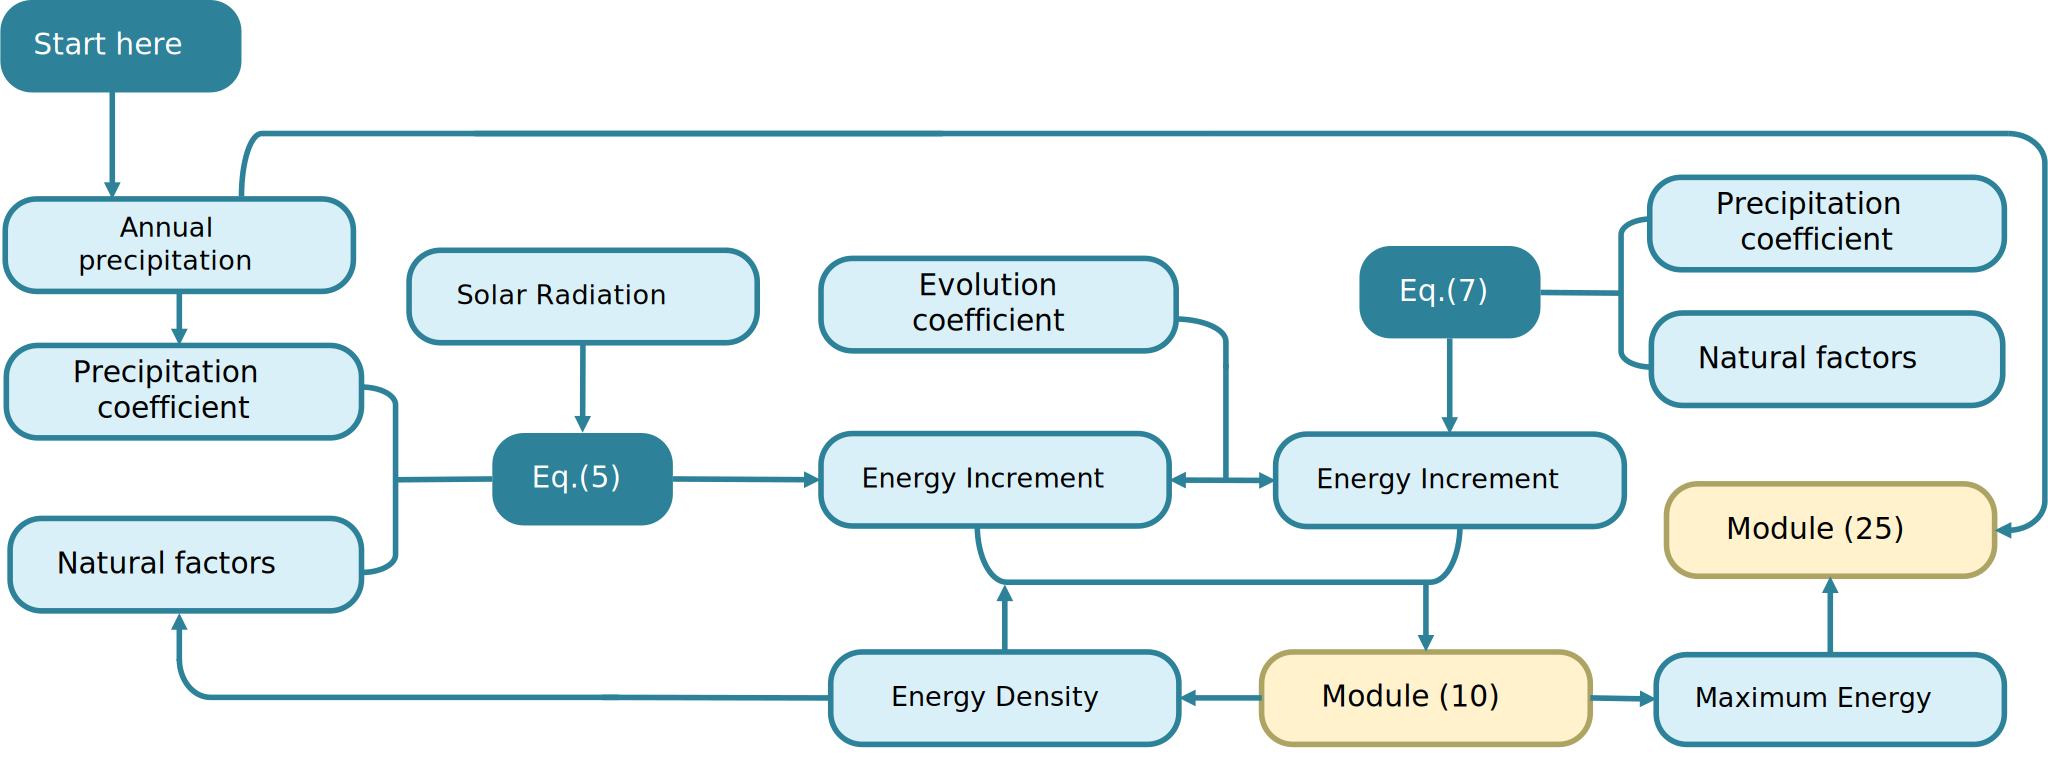
\includegraphics[width=0.92\textwidth]{easymcm/img/module.pdf}
	\caption{Overall analysis of the relationship of different parameters in this model}
    % 流程图,表示各个参数与方程之间的相互驱动关系
 \label{fig:work4}
\end{figure}

\vspace{-1cm}
\subsection{Sub-Model \uppercase\expandafter{\romannumeral1}: Singe-Plant Growth Model}
\vspace{-0.3cm}
In nature, plants obtain energy mainly through photosynthesis and respiration. Environmental factors, including light, humidity, temperature, pollution, and excessive drying, have both positive and negative influences on the plants' energy acquisition. To quantify these effects, our model treats plants and their environment as a system. At the same time, we also revised the parameters by the countervailing influence of the plant community on the environment. It predicts the fluctuation of the total energy of matter in a single plant community over time and provides the basis for subsequent multi-species plant community analysis.

\vspace{-0.5cm}
\subsubsection{Environmental Power On Plant Model}

\vspace{-0.5cm}
In the modeling process, we first represent the growth of the species in terms of total energy and calculate it as a function of time. We then combined photosynthesis and respiration to calculate the net increase in energy per week for the plant community. In the meantime, we have developed correlation functions for energy loss. 

\noindent$\blacktriangleright\ $\textbf{\small{Relationship between total energy and time}}

\vspace{-0.2cm}
According to the laws of biology, it is easy to calculate the annual energy of the community through net energy increment and energy loss. From this, we set the relationship between total energy and time as equation\eqref{eq:eq1}.

\vspace{-0.5cm}
\begin{shrinkeq}{-1ex}
	\begin{equation}
    \label{eq:eq1}
	  Q_i=Q_{i-1}+f_i-h_i
	\end{equation}
\end{shrinkeq}
\begin{itemize}
\vspace{-0.4cm}
\item[$\bullet$] \textbf{$Q_i$ }is the total material energy of a plant community in week $i$.
\vspace{-0.2cm}
\item[$\bullet$] \textbf{$f_i$ }is the net energy increment in a plant community in week $i$.
\vspace{-0.2cm}
\item[$\bullet$] \textbf{$h_i$ }is the net energy decrement in a plant community in week $i$.

\end{itemize}

\vspace{-0.2cm}
\noindent$\blacktriangleright\ $\textbf{\small{Energy increment in relation to photosynthesis and respiration}}

\vspace{-0.2cm}
Based on our assumption that photosynthesis and respiration are the primary sources of plant energy, and that photosynthesis yields significantly more energy than respiration, the model quantifies the energy increment of a plant population in terms of photosynthetic and respiratory. Additionally, taking into the research's reference to the "photosynthetic evolution" of plants{\cite{11}}, which implies the ability of plants to adjust their photosynthetic water and nitrogen uptake to varying environments, we introduced a plant genetic differentiation factor (FST) $G_1$ in the model to account for the non-linear expression of energy use during plant growth. Therefore, the expression formula of the final energy growth is as equation \eqref{eq:eq2}\eqref{eq:eq3}.

\begin{shrinkeq}{-1ex}
	\begin{equation}
    \label{eq:eq2}
	   f_i=G_1(v_{pi}+v_{bi})\cdot S
	\end{equation}
\end{shrinkeq}
\begin{shrinkeq}{-1ex}
	\begin{equation}
    \label{eq:eq3}
	   G_1 = 1+\frac{1}{\sigma_1\sqrt{2\pi}}e^{-\frac{(t-\mu_1)^2}{2\sigma_1^2}}
	\end{equation}
\end{shrinkeq}

\begin{itemize}
\vspace{-0.4cm}
\item[$\bullet$] \textbf{$v_{pi}$ }is photosynthetic energy production per $km^2$ in week $i$
\vspace{-0.2cm}
\item[$\bullet$] \textbf{$v_{bi}$ }is net respiratory energy yield per $km^2$ in week $i$
\vspace{-0.2cm}
\item[$\bullet$] \textbf{$G_1$ }is the multiplicative gain in energy production at week $i$ due to the evolutionary tendency of the plant. We fit it through a normal distribution model, where $\mu_1$ is the normal distribution mean, and $\sigma_1$ is the standard deviation.
\end{itemize}

\vspace{-0.6cm}
Then, let's discuss the quantitative energy expression of photosynthesis, which, as we have assumed, should take light radiation, temperature, atmospheric humidity, and soil moisture into consideration. The fact is that these factors occupy different importance at different levels of drought. There are researches{\cite{6}}{\cite{14}} that have given conclusions on this topic based on actual measurements. Therefore, we get the graph below.

% \vspace{-0.3cm}
\begin{figure}[htbp]
	\centering
	\includegraphics[width=0.8\textwidth]{easymcm/img/pollu.pdf}
	\caption{Relationship between natural factors and drought}
    % 雷达图,比较100mm和800mm降水的各个参数的贡献度
 \label{fig:work1}
\end{figure}

\vspace{-0.6cm}
The threshold for distinguishing a drought is an annual precipitation($R_{year}$) of less than $200mm$. Under this circumstance, as is vividly depicted in the above picture, weak transpiration in plants leads to reduced stomatal aeration and photosynthetic efficiency is particularly sensitive to soil moisture content($SH$) and solar radiation.  In this model, We measure the strength of solar radiation using the total energy of surface radiation received by the ground over the course of a week, which is denoted by the symbol $W_\phi$ 

While if annual precipitation is above $200mm$, the transpiration becomes relatively progressively more intense, bringing important photosynthetic water, inorganic salts, and other nutrients to photosynthesis. That is to say,  the dominant influences at this point are temperature, atmospheric humidity, and solar radiation. We use water vapor pressure deficit($VPD$) to evaluate these factors and portray it with equation \eqref{eq:eq4}.
\begin{shrinkeq}{-1ex}
	\begin{equation}
    \label{eq:eq4}
	   VPD=0.611 \exp(\frac{17.27 T}{T+237.3})(1-\frac{RH}{100\%})
	\end{equation}
\end{shrinkeq}

\begin{itemize}
\vspace{-0.4cm}
\item[$\bullet$] \textbf{$T$ }is average temperature for the week.
\vspace{-0.2cm}
\item[$\bullet$] \textbf{$RH$ }is the relative moisture for the week.
\vspace{-0.2cm}
\item[$\bullet$] The \textit{Constants} we use are from the paper{\cite{6}}.
\end{itemize}

\vspace{-0.2cm}
Based on the above analysis, we obtain an equation model to describe the energy production of photosynthesis in conjunction with the existing study{\cite{5}}. We use a modified rectangular hyperbola, and get the following set of equations to describe the photosynthetic.

\begin{shrinkeq}{-1ex}
	\begin{equation}
    \label{eq:eq5}
	   \left\{\begin{array}{l}
    v_{p} = k_{p1}v_{p1}+k_{p2}v_{p2}\\
   \\
    v_{p1}=\alpha_1\frac{1-\beta_1(VPD\cdot W_{\phi})}{1+\gamma_1(VPD\cdot W_\phi)} , \\
    \\
    v_{p2}=\alpha_2\frac{1-\beta_2(SH\cdot W_{\phi})}{1+\gamma_2(SH\cdot W_\phi)} , \\
   \\
    k_{p1} = (1-e^{-\frac{R_{year}}{200}})\cdot k_r,\\
   \\
    k_{p2} = e^{-\frac{R_{year}}{200}}\cdot (1-k_r),
\end{array}\right.
	\end{equation}
\end{shrinkeq}

\vspace{-0.2cm}
\begin{itemize}
\vspace{-0.2cm}
\item[$\bullet$] \textbf{$v_{p1}$ }is photosynthetic energy production per $km^2$ per week mainly affected by $VPD$.
\vspace{-0.2cm}
\item[$\bullet$] \textbf{$v_{p2}$ }is photosynthetic energy production per $km^2$ per week mainly affected by $SH$.
\vspace{-0.2cm}
\item[$\bullet$] \textbf{$k_r$ }is an index of plant drought resistance, which is used to adjust the proportion of time for photosynthesis under drought and non-drought conditions.
\vspace{-0.2cm}
\item[$\bullet$] \textbf{$k_{p1}$ }represents a measure of the energy production capacity of photosynthesis, where $VPD$ is the dominant factor influencing it.
\vspace{-0.2cm}
\item[$\bullet$] \textbf{$k_{p2}$ }is a measure of the energy production capacity of photosynthesis with $SH$ playing a dominant role.
\end{itemize}

\vspace{-0.5cm}
In order to simplify our model, we have assumed that there is a proportional relationship between the energy produced by respiration and that produced by photosynthesis, with this proportion being small. Accordingly, we have introduced a coefficient $k_p$ that is multiplied by the energy production of photosynthesis to express that of respiration. That is equation \eqref{eq:eq6}

\vspace{-0.2cm}
\begin{shrinkeq}{-1ex}
	\begin{equation}
    \label{eq:eq6}
	    v_b=kv_p
	\end{equation}
\end{shrinkeq}

\vspace{-0.2cm}
\noindent$\blacktriangleright\ $\textbf{\small{Energy Decrement }}

With the advent of global warming and increased industrialization in certain regions, plants in modern populations are not only subject to natural predators but also to environmental pollution. When considering the effects of pollution on plants, we have considered the two main categories of soil and water pollution and atmospheric pollution. 

With the advent of global warming and increased industrialization in certain regions, plants in 

\newpage

\begin{figure}[htbp]
\begin{minipage}[b]{0.5\linewidth}
 modern populations are not only subject to natural predators but also to environmental pollution. When considering the effects of pollution on plants, we have considered the two main categories of soil and water pollution and atmospheric pollution. Furthermore, as the plant grows to exceed its maximum energy density, its energy decrement per year will increase. Just as depicted in Figure\eqref{fig:figp}, air pollution, soil and water pollution, and natural losses during growth make up the three components of energy reduction.     
\end{minipage}
\hfill
\begin{minipage}[b]{0.45\linewidth}
\centering
\includegraphics[height=9\baselineskip]{easymcm/img/pollution.pdf}
\caption{Energy Decrement Factors}
\label{fig:figp}
\end{minipage}
\end{figure}

\vspace{-0.2cm}
We also consider the influence of the evolution of the plant and portray it with parameter $G2$. The definition of the energy decrement for a single plant population is as follows.
\vspace{-0.3cm}

\begin{shrinkeq}{-1ex}
	\begin{equation}
    \label{eq:eq7}
	    h_i=G_2(P_{wi}+P_{ai})+Q_{i-1}d
	\end{equation}
\end{shrinkeq}
\vspace{-0.1cm}
\begin{shrinkeq}{-1ex}
	\begin{equation}
    \label{eq:eq8}
	    G2 = 1-\frac{1}{\sigma_2\sqrt{2\pi}}e^{-\frac{(t-\mu_2)^2}{2\sigma_2^2}}
	\end{equation}
\end{shrinkeq}

\begin{itemize}
\vspace{-0.3cm}
\item[$\bullet$] \textbf{$P_{wi}$ }is the total energy lost per $km^2$ of water and soil pollution in week $i$.
\vspace{-0.2cm}
\item[$\bullet$] \textbf{$P_{ai}$ }is the total energy lost by air pollution per $km^2$ in week $i$.
\vspace{-0.2cm}
\item[$\bullet$] \textbf{$d$ }is natural energy loss ratio.
\vspace{-0.2cm}
\item[$\bullet$] \textbf{$G_2$ }is the multiplicative gain in energy decrement at week $i$ due to the evolutionary tendency of the plant. We fit it through a normal distribution model, where $\mu_2$ is the normal distribution mean, and $\sigma_2$ is the standard deviation.
\end{itemize}

\vspace{-0.2cm}
On the basis of the data in paper{\cite{8}}, we used $pH$ values to measure the degree of soil and water pollution, and the more the $pH$ Value deviates from neutral, the more harmful it is to plant growth For atmospheric pollution, we queried the common six atmospheric pollution gas components from {\cite{15}}as shown in the table below.
\vspace{-0.3cm}
% Table generated by Excel2LaTeX from sheet 'Sheet1'
\begin{table}[htbp]
  \centering
  \caption{Atmospheric concentrations of six common pollutant gases}
    \begin{tabular}{c|c|c|c|c|c|c}
    \hline
    \hline
		\makebox[0.28\textwidth][c]{\textbf{\textit{Ingredients}}}	&  \makebox[0.09\textwidth][c]{\textbf{\textit{$PM_{2.5}$}}}&
  \makebox[0.09\textwidth][c]{\textbf{\textit{ $PM_{10}$}}}&
  \makebox[0.09\textwidth][c]{\textbf{\textit{$CO$}}}&
  \makebox[0.09\textwidth][c]{\textbf{\textit{$NO_2$}}}&
  \makebox[0.09\textwidth][c]{\textbf{\textit{$SO_2$}}}&
  \makebox[0.09\textwidth][c]{\textbf{\textit{$O_3$}}}
	\\
    \hline
    \textbf{$Concentration$} $(ug/m^3)$ & $28$    & $49$    & $1000$  & $20$    & $9$     & $147$ \\
    \hline
    \hline
    \end{tabular}%
  \label{tab:addlabel}%
\end{table}%

From the table and literature review, we can conclude that the primary gases harmful to plants are $SO_2, NO_x, and CO$. So we use the total concentration($p$) of these gases as the indicator of atmospheric pollution.

Based on the above information, we can establish the mathematical function of plant mortality as below:

\begin{shrinkeq}{-1ex}
	\begin{equation}
    \label{eq:eq9}
    \left\{\begin{array}{l}
	P_w=K_1|PH-7|,\\
     P_a=K_2p,\\
     \end{array}\right.
    %  \left\{\begin{array}{l}
    %  PH_i=PH_{i-1}+b_1(1-e^{-\frac{Q|7-PH|}{RH\cdot T}}),\\
    %  \\
    %  p_i=p_{i-1}-b_2(1-e^{-\frac{QP}{RH\cdot T}}),
    % \end{array}\right.
	\end{equation}
\end{shrinkeq}

\begin{itemize}
\vspace{-0.2cm}
\item[$\bullet$] \textbf{$K_1$ }is the energy reduction per $km^2$ in week $i$ due to the deviation of pH from neutral. To simplify the model, we describe this effect as a linear process, with $K_1$ being a constant to be determined.
\item[$\bullet$]{$K_2$ }represents the reduction in energy per $km^2$ in week $i$ due to toxic gases. To simplify the model, we assume a linear relationship between the concentration of toxic gases and the reduction in energy, with $K_2$ as a constant that needs to be determined.
\end{itemize}

\vspace{-0.2cm}
\noindent$\blacktriangleright\ $\textbf{\small{Stage summary}}

So we can have a stage summary of the module of Environmental Power On Plant shown below. 

\begin{shrinkeq}{-1ex}
	\begin{equation}
    \label{eq:eq10}
    \left\{\begin{array}{l}
	Q_i=Q_{i-1}+f_i-h_i\\
    \\
    f_i=G_1(v_{pi}+v_{bi})\cdot S,\\
    \\
    h_i=G_2(P_{wi}+P_{ai})+\rho_{i-1}d
    \end{array}\right.
	\end{equation}
\end{shrinkeq}

The specific formulas for these parameters have been shown in the above contents.

\vspace{-0.5cm}
\subsubsection{Plant Reaction to the Environment}

\vspace{-0.4cm}
Based on our literature research, it has been noted that plants have significant countervailing effects on the environment, including the impact on atmospheric temperature and humidity, the mitigation of pollution, and the retention of soil moisture. Collectively, these efforts by plants generally contribute to creating a more favorable environment for their growth.

\noindent$\blacktriangleright\ $\textbf{\small{Natural factors }}

In summer, the trees absorb, reflect and scatter a large amount of solar energy, reducing the rate of warming at ground level. In winter, the trees wither, but their branches still act as a barrier to air currents, reducing wind speed and exerting an insulating and moisturizing effect{\cite{1}}.
One research{\cite{9}} carried out a large number of practical observations to examine the processes by which flora affects temperature. The results show that precipitation and plant density play a more significant role in this process. Based on their data, we get the following equation:

\begin{shrinkeq}{-1ex}
	\begin{equation}
    \label{eq:eq11}
    \rho=\frac{Q}{S}
	\end{equation}
\end{shrinkeq}


\begin{shrinkeq}{-1ex}
	\begin{equation}
    \label{eq:eq12}
    \varDelta T=
    \left\{\begin{array}{l}
	(-0.48\cdot\frac{400+R_{year}}{400}-0.28)\rho, \quad R_{year}\in(0,400]\\
 \\
    (-0.62\cdot\frac{400+R_{year}}{400})\rho,     \qquad \qquad R_{year}\in(400,800]\\
\\   
    (-0.86\cdot\frac{R_{year}}{400})\rho,       \qquad  \qquad \qquad R_{year}\in(800,2500]
    \end{array}\right.
	\end{equation}
\end{shrinkeq}

\begin{itemize}
\vspace{-0.2cm}
\item[$\bullet$] \textbf{$\rho$ }is current plant energy density.
\end{itemize}

\vspace{-0.2cm}
In addition to influencing atmospheric temperatures, good plant distribution also enhances solar radiation through reflection from the top of the tree canopy{\cite{9}}. We can describe this in the following method: 

\begin{shrinkeq}{-1ex}
	\begin{equation}
    \label{eq:eq13}
    \alpha=0.1-e^{-\frac{\alpha }{\rho}} 
	\end{equation}
\end{shrinkeq}
\begin{shrinkeq}{-1ex}
	\begin{equation}
    \label{eq:eq14}
    W_\phi=W_{\phi 0}(1-\alpha)
	\end{equation}
\end{shrinkeq}

\begin{itemize}
\vspace{-0.2cm}
\item[$\bullet$] \textbf{$\alpha$ }is change in albedo value.

\vspace{-0.2cm}
\item[$\bullet$] \textbf{$W_{\phi 0}$ }is the original energy of surface radiation received by the ground.
\end{itemize}

The paper also studied the change in humidity over time{\cite{9}}, and we build the influence of flora on humidity on the basis of it. The formula is shown as below.

\begin{shrinkeq}{-1ex}
	\begin{equation}
    \label{eq:eq15}
    K_{RH}=\frac{k_5}{1+e^{-\frac{T\rho}{T+C}}}
	\end{equation}
\end{shrinkeq}
\begin{shrinkeq}{-1ex}
	\begin{equation}
    \label{eq:eq16}
    RH=K_{RH}\cdot RH_0
	\end{equation}
\end{shrinkeq}

\begin{itemize}
\vspace{-0.2cm}
\item[$\bullet$] \textbf{$k_5$ }is atmospheric humidity conversion factor.

\vspace{-0.2cm}
\item[$\bullet$] \textbf{$K_{RH}$ }is atmospheric humidity correction factor.

\vspace{-0.2cm}
\item[$\bullet$] \textbf{$RH_0$ }is original relative humidity.

\vspace{-0.2cm}
\item[$\bullet$] \textbf{$C$ }is pending constants.
\end{itemize}
\vspace{-0.3cm}

There are also data{\cite{8}} showing that as the density of the flora increases, its effect on soil and water conservation is enhanced. We express this effect as an enhancement and retention of soil moisture. Here we use equation\eqref{eq:eq16}\eqref{eq:eq17} to depict this effect.

\begin{shrinkeq}{-1ex}
	\begin{equation}
    \label{eq:eq17}
    SH=K_{SH}\cdot SH_0
	\end{equation}
\end{shrinkeq}
\begin{shrinkeq}{-1ex}
	\begin{equation}
    \label{eq:eq18}
    K_{SH}=\frac{k_4}{1+e^{-\rho}}
	\end{equation}
\end{shrinkeq}

\begin{itemize}
\vspace{-0.2cm}
\item[$\bullet$] \textbf{$k_4$ }is soil moisture conversion factor.

\vspace{-0.2cm}
\item[$\bullet$] \textbf{$K_{SH}$ }is soil moisture correction factor.

\vspace{-0.2cm}
\item[$\bullet$] \textbf{$RH_0$ }is original soil moisture.
\end{itemize}

\vspace{-0.5cm}
\noindent$\blacktriangleright\ $\textbf{\small{Mitigating pollution}}

The research{\cite{7}} collected data on how the flora mitigates pollution, and the conclusion is flora can achieve this goal to an excellent extent. Therefore, we get the following formula.

\begin{shrinkeq}{-1ex}
	\begin{equation}
    \label{eq:eq19}
     \left\{\begin{array}{l}
     PH_i=PH_{i-1}+b_1(1-e^{-\frac{\rho |7-PH|}{RH\cdot T}}),\\
     p_i=p_{i-1}-b_2(1-e^{-\frac{\rho P}{RH\cdot T}}),
    \end{array}\right.
	\end{equation}
\end{shrinkeq}

\begin{itemize}
\vspace{-0.2cm}
\item[$\bullet$] \textbf{$b_1$ }is $pH$ value correction factor.

\vspace{-0.2cm}
\item[$\bullet$] \textbf{$b_2$ }is pollutant gas concentration correction factor.
\end{itemize}
% \vspace{-1.8cm}
% \vspace{0.8cm}
\subsubsection{Model Combination and Determining the Constansts' Values}

Different plants have varying abilities to resist drought. In the test results presented in the article{\cite{6}}, the osmanthus tree, camphor tree, and Masson pine have different degrees of response to drought. By monitoring the stem water flow, trunk sap flow, soil composition, and various meteorological factors of the trees, the researchers quantified the tree transpiration response to environmental factors. This reveals the differences in plants' drought resistance abilities.

In our plant energy metabolism model, we need to confirm the parameters in the equation based on the drought resistance and growth characteristics of different plants. Considering the reliability of the results, we used the sensitivity in the paper as a reference for the parameters $k_{p1}$ and $k_{p2}$ in the expression of photosynthesis in the model, which mainly affect the relationship between photosynthesis rate and drought severity. The mean value $\mu$ in the genetic factor G1 can also be determined by comparing changes in photosynthesis in trees during drought periods. $\mu$ is used to quantify the plant's ability to improve photosynthesis, i.e., the time when the photosynthesis rate reaches its peak.

% \vspace{-0.3cm}
\begin{figure}[htbp]
	\centering
	\includegraphics[width=1\textwidth]{easymcm/img/Tree species.pdf}
	\caption{The degree of response to drought varies among different tree species}
    % 三种树木的测试表格,用于确认参数
 \label{fig:degree}
\end{figure}
% \vspace{-0.3cm}

From the radar chart in figure \eqref{fig:degree}, we can see that the osmanthus tree is the most sensitive to soil moisture content under drought conditions, which confirms our description that soil moisture content is the most important factor in drought conditions. 

The value of $k_{p1}$ for the osmanthus tree is much larger than that of $k_{p2}$, because in normal conditions, the osmanthus tree is much more sensitive to solar radiation than the camphor tree and Masson pine in the same period. This indicates that the osmanthus tree has a stronger drought resistance ability, with more vigorous transpiration, resulting in a higher value of $k_{p1}$. The larger value of $\mu$ compared to the other two trees indicates that the genetic factor G1 of the osmanthus tree can increase the time for better enhancement of photosynthesis.

The other parameters, such as natural death rate $d$ and pollution factors $P_a$ and $P_w$, are calculated using uniform parameters and are not changed based on the characteristics of different plants.

\subsection{Sub-Model \uppercase\expandafter{\romannumeral2}: Multi-Plant Interaction Model}

According to classical ecological theory, higher species diversity leads to a greater complementarity effect of ecological niches. The ecological niche complementarity effect refers to the divergence and complementarity between the ecological niches of different organisms in an ecosystem, which implies temporal and spatial differences in resource use. Based on this, we developed a competition-dependence model between species.

After the discussion in the previous section, we constructed a single-class species growth model that analyzes the relationship between the net energy increase ($f-h$) and the total material energy ($Q$) of a species. Here we show this equation again as below.
\begin{shrinkeq}{-1ex}
	\begin{equation}
    \label{eq:eq31}
	  Q_i=Q_{i-1}+f_i-h_i
	\end{equation}
\end{shrinkeq}

To take command of the Logistic Model, this equation should first be rewritten into the following module:

\vspace{-0.2cm}
\begin{shrinkeq}{-1ex}
	\begin{equation}
    \label{eq:eq32}
	  Q_{i+1}=\alpha \cdot Q_{i}\cdot(1-\frac{Q_i}{Q_{max}})
	\end{equation}
\end{shrinkeq}

Here, $Q_{max}$ is the limiting value of $Q$, which is proved that can be calculated in section 3.2.3. $\alpha$ can be described as the equation \eqref{eq:eq33}
\begin{shrinkeq}{-1ex}
	\begin{equation}
    \label{eq:eq33}
	  \alpha= Q_{max} \cdot \frac{(f_{i}-h_{i}) + Q_{i}}{Q_{max}Q_{i}-{Q_{i}}^2}
	\end{equation}
\end{shrinkeq}

We set the species competing in this model as two categories: drought-resistant and non-drought-resistant plants, and let their total energy be $Q_1$ and $Q_2$ respectively, and let the coefficient covariate of competition between the two categories of species be $S_i$. Considering the interaction between the two categories of species, we bring in equation \eqref{eq:eq32} to obtain the new quantitative relationship as follows:

\begin{shrinkeq}{-1ex}
	\begin{equation}
    \label{eq:eq34}
	\left\{\begin{array}{l}
     Q_{i+1,1}=\alpha Q_{i,1}(1-\frac{Q_{i,1}}{Q_{max,1}}-S_i\frac{Q_{i,2}}{Q_{max,2}})\\
     \\
    Q_{i+1,2}=\alpha Q_{i,2}(1-\frac{Q_{i,2}}{Q_{max,2}}-S_i\frac{Q_{i,1}}{Q_{max,1}})
    \end{array}\right.
	\end{equation}
\end{shrinkeq}

\vspace{0.2cm}
Reciprocal effects exist between tree species. For example, different tree species have different depths of roots. In times of drought, deep-rooted trees can absorb water from the deep soil to the top soil, providing water to shallow-rooted trees and thus increasing their resistance to drought. This reciprocal interaction between species is important for forests to withstand drought. 

The ecological theory of the 'stress gradient hypothesis' suggests that the strength and importance of reciprocal interactions between species increases with increasing environmental stress and that the strength and importance of competitive interactions decrease with increasing environmental stress. As the degree of water stress increases, competition between tree species decreases or reciprocity increases, and the contribution of tree species diversity to forest resistance increases significantly. The relationship between tree species under drought stress is dominated by reciprocity.
Therefore, combined with the data from the research {\cite{16}}, we can portray $S_i$ as a function of the degree of drought by equation \eqref{eq:eq35}.

\newpage
\begin{shrinkeq}{-1ex}
	\begin{equation}
    \label{eq:eq35}
	  S_i = \beta (\frac{3}{4}-\frac{1}{1+exp(\gamma(R_{year}-R_{drought}))})
	\end{equation}
\end{shrinkeq}

\begin{itemize}
\vspace{-0.2cm}
\item[$\bullet$] \textbf{$\beta$, $\gamma$} is the two factors to be determined. 

\vspace{-0.2cm}
\item[$\bullet$] \textbf{$R_{drought}$} is the boundary between arid and non-arid weather. In Section 3.2 we have known it is $200mm$ of precipitation in a single year.
\end{itemize}

\vspace{-0.5cm}
Here, we take precipitation as the independent variable and the image of the $S_i$ function is S-shaped, with reciprocity dominating in the drought case when $S_i < 0$, and competition dominating in the non-drought case when $Si > 0$. 

\begin{figure}[htbp]
	\centering
	\includegraphics[width=0.5\textwidth]{easymcm/img/Si-Ryear.pdf}
	\caption{The relationship between the number of species with $S_i$}
 \label{fig:si}
\end{figure}

\vspace{-0.3cm}
From the graph, we can conclude that the number of species ($N$) makes a difference in this circumstance, as each species is subject to competition or reciprocity from $(N-1)$ other species, so equation \eqref{eq:eq35} should be modified. After this, we reach our conclusion about the Multi-Plant Interaction Model.

\begin{shrinkeq}{-1ex}
	\begin{equation}
    \label{eq:eq36}
    \left\{\begin{array}{l}
     Q_{i+1,1}=\alpha Q_{i,1}(1-\frac{Q_{i,1}}{Q_{max,1}}-S_i\frac{Q_{i,2}}{Q_{max,2}})\\
\\
    Q_{i+1,2}=\alpha Q_{i,2}(1-\frac{Q_{i,2}}{Q_{max,2}}-S_i\frac{Q_{i,1}}{Q_{max,1}})\\
\\
    S_i = \beta(N-1)(\frac{3}{4}-\frac{1}{1+exp(\gamma(R_{year}-R_{drought}))})
    \end{array}\right.
	\end{equation}
\end{shrinkeq}

\vspace{-0.5cm}
\subsection{Indicators: Species Richness and Drought Resistance}
\vspace{-0.3cm}
To better measure the development of the community, two evaluation indicators are established, namely species richness and drought resistance of the plant community.

To assess the drought resistance($R_t$) of a species or community and distinguish between drought-resistant and non-drought-resistant plants, we introduce a covariate. Considering that the degree of drought is measured by precipitation and that total biological energy characterizes the growth of plants, we used these two parameters to calculate this indicator, and it is defined as equation\eqref{eq:eq37}. 

\begin{shrinkeq}{-1ex}
	\begin{equation}
    \label{eq:eq37}
    R_t = Q_{max}\frac{dR_{year}}{dQ_{max}}
	\end{equation}
\end{shrinkeq}

\vspace{0.2cm}
Here, we calculate the precipitation change required for a given relative change in the maximum biological energy of the subject under a certain precipitation amount. In this method, $R_t$ positively represents plant drought resistance, meaning that the greater the $R_t$, the more drought resistant the plant community is.  

 To measure the biodiversity in a population, We use the formula for calculating species richness proposed by Margalef in 1958, which is displayed in equation\eqref{eq:eq38},where $i$ mean the $i-th$ species of plant, and $SR$ represents species variety within a unit size space.

\begin{shrinkeq}{-1ex}
	\begin{equation}
    \label{eq:eq38}
    SR = \frac{N-1}{ln(\Sigma_i Q_{i,max})}
	\end{equation}
\end{shrinkeq}

\vspace{-0.5cm}
\section{Model Application}
\vspace{-0.3cm}
\subsection{Climate Data}

\begin{figure}[htbp]
	\centering
	\includegraphics[width=0.8\textwidth]{easymcm/img/map.pdf}
	\caption{Diagram of flora in different climate zone}
 \label{fig:map}
\end{figure}


To apply our model and answer the relevant questions, we have selected regions characterizing each of the three wetting levels, as shown in figure\eqref{fig:map}.By measuring the energy variation in areas of three different levels of aridity, we can summarize the important rules of species diversity and drought resistance for the survival and reproduction of plant populations. 

The Amazon rainforest is a well-known area with high species diversity and energy density of plant populations, while the Karoo National Park in South Africa is mainly composed of shrubs and grasses with strong drought resistance. Witjira National Park in central Australia is located in desert and semi-desert regions, where vegetation is relatively sparse, but plants have adapted to extreme arid conditions. Therefore, the plant populations in these three areas are extremely valuable for research.

To simplify the simulation, we calculate weekly data using monthly data for the region, obtaining data on humidity, soil moisture, precipitation, temperature, and surface solar radiation energy. This provides the database for our subsequent simulation analysis.
\newpage

\vspace{-0.3cm}
\begin{figure}[htbp]
	\centering
	\includegraphics[width=0.8\textwidth]{easymcm/img/parameter.pdf}
	\caption{Temperature, humidity, soil moisture,
            surface solar radiation, and precipitation data in 2019}
 \label{fig:para}
\end{figure}

As shown in picture \eqref{fig:para}, we collect the data of natural factors in our model. And based on these data, we calculate the water vapor pressure deficit($VPD$) according to equation \eqref{eq:eq4}. We plot it in graph\eqref{fig:var}. At last, we calculate the $Q_{max}$ in $1 km^2$, which is shown in picture \eqref{fig:qlast}

\begin{figure}[htbp]
	\centering
	\begin{minipage}[t]{0.5\textwidth}
		\centering
		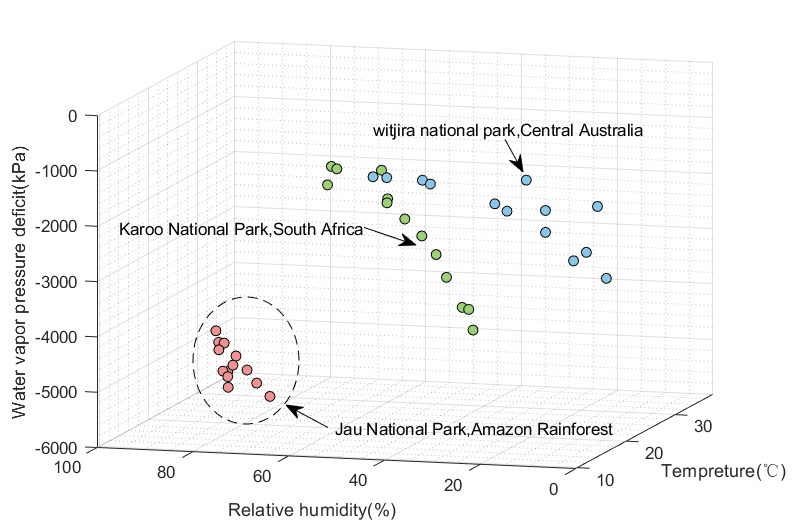
\includegraphics[width=1\textwidth]{easymcm/img/VPD.pdf}
		\caption{Water vapor pressure deficit}\label{fig:var}
	\end{minipage}
	\begin{minipage}[t]{0.4\textwidth}
		\centering
		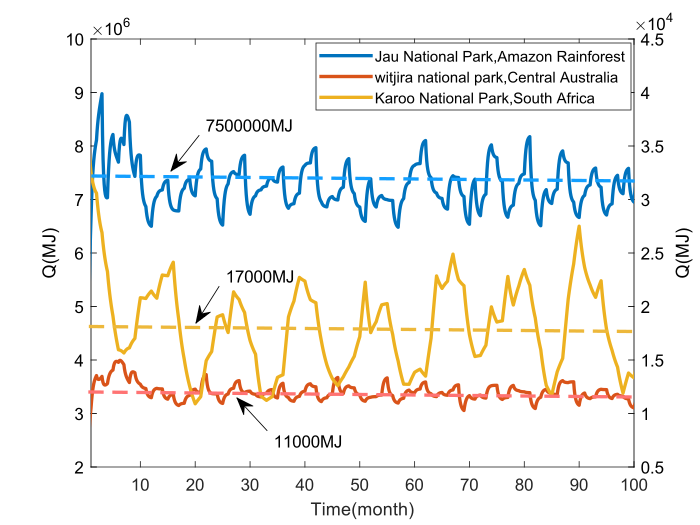
\includegraphics[width=0.98\textwidth]{easymcm/img/Qlast.pdf}
		\caption{$Q_{max}$ in three places}\label{fig:qlast}
	\end{minipage}
\end{figure}

In preprocessing the data for the three regions, it is evident that the water vapor pressure deficit in the Amazon rainforest community is significantly larger than in the arid and non-arid regions. Additionally, various environmental factors show strong seasonality. In Figure 11, we can observe that the total energy $Q$ exhibits strong oscillations, with the energy per square kilometer reaching as high as $7.5\times 10^6MJ$ with an amplitude of $10^6MJ$ in the Amazon rainforest community, while in South Africa and central Australia, the total energy is only $(1\sim 1.2)\times 10^5MJ$, with relatively smaller oscillations. From this, we can conclude that the energy density in humid areas is much higher than in arid areas, and the amplitude of oscillation is also greater.

\subsection{Number of different species}

When the proportion of drought-resistant plant species in the community is a certain proportion $k$, we can find the expected value of the amount of drought-resistant plant species in the community when the amount of species is $N$. Thus the expected value of the amount of drought-resistant plant species in the community is $kN$. Here, we set $k=0.07$.

We assume that there is no difference between plants under normal conditions (annual precipitation reaches $600mm$) other than their drought resistance. That is to say, the total bioenergy of each plant is equal. Besides, we exclude the influence of pollution. We take the total bioenergy of drought-resistant and non-drought-resistant plants under normal conditions as the initial value and use the Multi-Plant Interaction Mode to obtain the total bioenergy of drought-resistant and non-drought-resistant plants and the total bioenergy of the community over time. 

Here, we set annual precipitation as $R_{drought}$, which is $200mm$. The relationship between $R_t$ and species volume $N$ is shown below.

\begin{figure}[!htbp]
	\centering
	\begin{minipage}[t]{0.45\textwidth}
		\centering
		\includegraphics[width=1\textwidth]{easymcm/img/RT-N.pdf}
		\caption{Relationship between $R_t$ and $N$}
        \label{fig:rt-n}
	\end{minipage}
	\begin{minipage}[t]{0.45\textwidth}
		\centering
		\includegraphics[width=1\textwidth]{easymcm/img/Tree adress.pdf}
		\caption{Relationship between $SR$ and $N$}
        \label{fig:treeadd}
	\end{minipage}
\end{figure}


\vspace{-0.5cm}
From graph\eqref{fig:rt-n}, we can obtain that, without considering the type of plant species, a mutation process starts to occur in the plant population when the number of species is 8 and the plants are more resistant to drought. Thereafter, as the $N$ grows, there is a larger increase in $R_t$ when $kN$ equals an integer. Overall, plant populations begin to develop drought resistance when $N=8$, and subsequently drought resistance increases as $N$ increases.

While in graph\eqref{fig:treeadd}, as the three straight lines show, the more arid the area, and taking into account the competitive effects between species, the fewer species would be needed to achieve the same species richness. At the same time, plants at higher levels of aridity can achieve higher species richness for the same number of species. This result is also consistent with the findings in study{\cite{12}}.

\subsection{Composition of the flora types}

In accordance with Assumption 1, we compare the effects of three main types of trees, shrubs, and herbs on the two indicators and total energy. We do the simulation with data of central Australia and exclude the influence of pollution. 

\begin{figure}[htbp]
	\centering
	\begin{minipage}[t]{0.45\textwidth}
		\centering
		\includegraphics[width=1\textwidth]{easymcm/img/Rt-D-type.pdf}
		\caption{Relationship among $R_t$, $SR$, type}
  \label{fig:type}
	\end{minipage}
	\begin{minipage}[t]{0.45\textwidth}
		\centering
		\includegraphics[width=0.98\textwidth]{easymcm/img/Qmax-month.pdf}
		\caption{Relationship between $Q_{max}$ and type}\label{fig:qmon}
	\end{minipage}
\end{figure}

Analysis of graph \eqref{fig:type} shows that herbaceous plants are able to achieve the greatest drought resistance when species richness is certain, while trees have the lowest drought resistance. At the same time, to achieve the same level of drought resistance, the species richness required for a group of species is, in descending order, trees, shrubs and herbs. Besides, from graph\eqref{fig:qmon} we also tell that Grass grows best. We can therefore conclude that herbs are the most drought resistant, followed by shrubs, and trees the least.
\vspace{-0.5cm}
\subsection{Frequency and variation of drought}
\vspace{-0.3cm}
When calculating the effect of drought frequency on the growth of plant communities, we designed the amount of precipitation over a period of time by using a sine function. Through calculating the results of population energy affected by this factor for different numbers of species, and the relationship between population size and drought resistance and drought frequency, we completed the plotting of Figure \eqref{fig:fre}.

\begin{figure}[htbp]
	\centering
	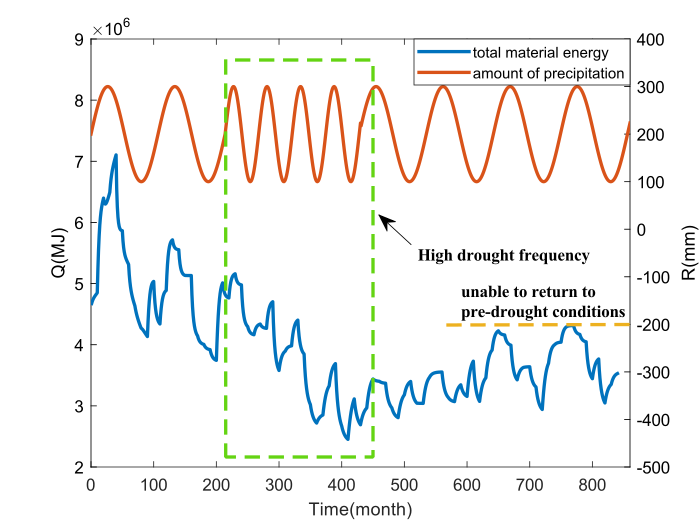
\includegraphics[width=0.8\textwidth]{easymcm/img/fre.pdf}
	\caption{Influence of drought frequency. \textit{Left graph} depicts the influence of it on the total energy with their species numbers are $15$ and $45$ respectively. \textit{Right graph} describes the influence of it on the drought resistance.}
 \label{fig:fre}
\end{figure}

\vspace{-0.5cm}
With respect to the graph on the right, when the frequency of drought decreases, the energy of the multispecies community follows a U-shape, first decreasing and then increasing. The energy of the lesser species communities then decreases. This is explained by the fact that the higher the frequency of drought, the greater the tendency for plants to become more drought resistant. However, when a community has a wide range of plants, it has a greater capacity to carry drought. Therefore, when drought frequency is not very high, the community is more inclined to cope with drought by reducing its scale. In addition, reciprocity between plants increases the total bioenergy of the community, and reciprocity between multiple species is stronger at the same drought frequency, so the more species species there are, the more drought resistant they are.

In the picture on the left, after a higher frequency of drought, the community energy of only $15$ plant species has difficulty returning to its previous level, while the community energy of $45$ plant species returns to normal. We therefore suggest that when species numbers are low, high frequencies of drought can cause irreversible damage to the community. This may be because the damaging effects of drought outweigh the growth of plant drought resistance. Multi-species communities, on the other hand, are inherently more drought resistant and are therefore able to return to normal after higher frequency droughts. Thus, when droughts are less frequent, the greater the number of species, the greater the total energy of the species.

We then measured the impact of changes in arid areas on the total energy of the community by varying the proportion of the total area that is arid (using data from South Africa) and non-arid (using data from the Amazon rainforest). The result is that total community energy decreases with an increasing proportion of drought areas.
\vspace{-0.5cm}
\subsection{Pollution and habitat reduction}
To gauge the effect of pollution on plant community development, we simulated the parameters related to the reduction in plant energy and the results are shown in Figure\eqref{fig:3d}.
\vspace{0.1cm}
\begin{figure}[htbp]
	\centering
	\includegraphics[width=0.6\textwidth]{easymcm/img/3d.pdf}
	\caption{Influence of pollution.}
 \label{fig:3d}
\end{figure}
\vspace{-0.3cm}
As can be seen from the figure, $pH$ has little effect on the maximum total energy, with the more acidic the soil, the smaller the total energy. In contrast, the concentration of noxious gases has a greater effect on the maximum total energy, with the maximum total energy changing by more than a factor of 10 for every 1 $mg/m^3$ increase. Therefore, deviations from the actual pollution factor do matter.

Similar to pollution, habitat reduction has a side effect on total maximum energy. Our calculation shows that smaller habitats fluctuate at lower energy and have smaller peaks when the total energy reaches its peak, resulting in less adaptive to drought. It can therefore be concluded that for plant communities, the larger the habitat, the better it is for the plant community.

\vspace{-0.5cm}
\subsection{Suggestions on the long-term viability of a plant community}
\vspace{-0.2cm}
Based on the above analysis, we give the following suggestions for the long-term development of the plant community.


\begin{itemize}
\vspace{-0.4cm}
\item[$\bullet$] \textbf{Increase the variety of plants}

\vspace{-0.2cm}
When planted with a wide range of plants, the community will be more drought resistant to higher frequencies of drought than a community with a lower number of species, as shown in our previous analysis. Plant communities with multiple populations are therefore more likely to be benign in the long term.


\item[$\bullet$] \textbf{Rational dense planting}

\vspace{-0.2cm}
According to our analysis, when the density is too high, it increases the energy loss of the population. In addition, reasonably dense planting can make better use of soil nutrients to improve the plant growth environment and increase the plants' ability to absorb nutrients.

\vspace{-0.2cm}
\item[$\bullet$] \textbf{Reducing land reclamation and eliminating deforestation}

\vspace{-0.2cm}
Policies and regulations for vegetation protection need to be developed, while publicity and education need to be strengthened to raise public awareness of vegetation protection. In addition, monitoring and assessment of vegetation need to be strengthened to identify and solve problems faced by vegetation in a timely manner. For example, a forest resources census can be carried out to understand the distribution, area, type, and growth of forests, and to identify and deal with problems such as deforestation and fires in a timely manner.
\end{itemize}
\vspace{-0.5cm}

Taking into account the previous analysis, we believe that our measures can bring the following benefits to the larger environment.
\vspace{-0.2cm}

\begin{itemize}
\vspace{-0.2cm}
\item[$\bullet$]  A reduction in pollution while making the air more humid and having more ions to trap airborne pollution particles.
\vspace{-0.2cm}
\item[$\bullet$] An increase in surface albedo, which reduces the evaporation of water from the land by sunlight and acts as a water and soil anchor.
\vspace{-0.2cm}
\item[$\bullet$] Reduction in temperature, which greatly reduces the warming caused by the temperature effect today
\end{itemize}

\vspace{-1cm}
\section{Sensitivity Analysis}
\vspace{-0.5cm}
In real-life situations, statistical data is often inaccurate and there may be biases in the input to our model. These biases can impact the results of our model. To test the robustness of our model, in this section, we will analyze the sensitivity of our decision model in the analysis.

\vspace{-0.5cm}
\subsection{Sensitivity Analysis of plant drought resistance}

\vspace{-0.3cm}

The drought resistance of different plants plays a key role in our model, which can lead to misjudgment of the best management plan, resulting in an imbalance of the various plants in the forest. Drought resistance affects the rate of energy growth of plants. To measure the extent to which this affects the model, we set a fluctuating value of $5\%$ for it and calculate the total energy.

\begin{figure}[htbp]
	\centering
	\includegraphics[width=0.45\textwidth]{easymcm/img/sens.pdf}
	\caption{Energy changes at different drought resistance coefficient}
 \label{fig:figkr}
\end{figure}

As shown in Fig\eqref{fig:figkr}, when $k_r$ fluctuates, the total energy storage of the plant community fluctuates slightly. When $k_r$ fluctuates by 5\%, the fluctuation of stable energy storage is about 1.67\%. Therefore, We can therefore conclude that our model is robust to $k_r$.

\vspace{-0.5cm}
\subsection{Sensitivity Analysis of natural factors}
\vspace{-0.5cm}
In addition to the drought resistance factor $k_r$, there are many unstable factors in our model. In order to verify the robustness of the model, we will mainly use four natural factors as objects and use heat maps for sensitivity analysis.

\vspace{-0.2cm}
\begin{figure}[htbp]
	\centering
	\includegraphics[width=0.9\textwidth]{easymcm/img/Heat.pdf}
	\caption{Energy when natural factors fluctuate}
 \label{fig:fignaf}
\end{figure}

\vspace{-0.3cm}
In these two figures, it is obvious that, except for the surface solar radiation, the other three environmental factors reach the maximum total energy value near the center. The higher the solar radiation, the higher the total energy that can be achieved, until it reaches saturation at 160 $MJ/km^2\cdot week$.When the relative humidity is between $30\% \sim 40\%$, the soil moisture content is around $50\%$, and the temperature is between 15°C to 35°C, the total energy is at its maximum. When all parameters are changed, there is no sudden change phenomenon, and the peak position is obvious and consistent with the actual situation. This indicates that our model has good robustness.

\section{Model Evaluation and Further Discussion}

\vspace{-0.5cm}
\subsection{Strengths}

% \vspace{-0.3cm}
\begin{itemize}
\item[$\bullet$] \textbf{Highly realistic }

Our model is constructed with extensive reference to actual research data and has a strong value for realistic assessment. This allows us to obtain more accurate results when bringing in actual or hypothetical scenarios. In other words, by closely incorporating real-life data, our model is able to better predict how plant communities will respond to drought in reality.

\item[$\bullet$] \textbf{Robust Model }

As shown in our sensitivity analysis results, our model has strong robustness under both fluctuations in drought resistance of the single plant and natural factors. Therefore, we believe that our model has good robustness.

\item[$\bullet$] \textbf{Strong Interpretability }

In creating our model, our step-by-step approach to building the model allowed us to gain a better understanding of the complex relationship between plant species and their drought resilience. By focusing on the individual components and gradually building the model, we were able to consider the interactions between the various factors in a more nuanced and detailed manner. This gives our model a more powerful interpretability.

\item[$\bullet$] \textbf{Comprehensiveness }

We take into account the influence of a variety of factors when exploring plant growth. For example, we not only consider the role of atmospheric moisture but also explore how soil moisture affects plant communities. More importantly, we have combined a number of factors and considered them separately for different plant species, which increases the complexity of the model to some extent, but also makes our model more universal.


\end{itemize}

However, there are weaknesses in the proposed models:

\vspace{-0.5cm}
\subsection{Weaknesses}
\vspace{-0.3cm}
\begin{itemize}

\item[$\bullet$] \textbf{Limited weather types}

In order to target the discussion of plant communities in relation to drought adaptation, we do not consider other extreme weather conditions. However, chances are that a superposition of different levels of weather extremes may end up with different curves of plant growth trends.

\item[$\bullet$] \textbf{Simple Indicator of benefits on environment}

In assessing when the environment starts to pay off, the metric we use is species diversity. However, the real-world measure of environmental gain can be far more complex than this.

\end{itemize}

\vspace{-0.5cm}
\subsection{Further Improvements}

\vspace{-0.3cm}
If time permits, we will refine our model from the following three points:

\begin{itemize}

\item[$\bullet$] We will build a larger database of plants and drought environments to allow a more accurate fit of our model parameters.

\item[$\bullet$] We will make a more systematic assessment of the effects of environmental pollution on plants and analyze the importance of phytoremediation in environmental pollution.

\item[$\bullet$] We will enrich the variety of weather extremes considered. The robustness of our model will be more thoroughly evaluated and optimized by considering the effects of multiple climate extremes on plant communities

\end{itemize}
\newpage
\begin{thebibliography}{99}
	\vspace{-0.5cm}
    \bibitem{1}{Liu, D., Wang, T., Peñuelas, J., \& Piao, S. (2022). Drought resistance enhanced by tree species diversity in global forests. Nature Geoscience, 15(10), 800-804.}

	\bibitem{2}\url{https://www.ugaoo.com/blogs/gardening-basics/photosynthesis-and-respiration}
    \bibitem{3}\url{https://education.nationalgeographic.org/resource/photosynthesis/}

    \bibitem{4}{YE Z P. A review on modeling of responses of photosynthesis to light and CO2[J]. Chinese Journal of Plant Ecology, 2010, 34(6): 727.}

    \bibitem{5}{Ye Z, Zhao Z. A modified rectangular hyperbola to describe the light-response curve of photosynthesis of Bidens pilosa L. grown[J]. Frontiers of Agriculture in China, 2010, 4(1): 50.}


    \bibitem{6}{Dai Junjie, et al. Response and simulation of transpiration of typical trees to environmental factors[J]. Resources and Environment in the Yangtze Basin, 2021.}

    \bibitem{7}{Nie Lei, Deng Zhihua, Chen Qibo, Chang Yushan. Effect of Kunming urban forest on atmospheric $SO_2$ and $NO_X$ purification[J]. Western Forestry Science,2015,44(04):116-120.}

    \bibitem{8}{Zhang, L.F.,Hu, H.L.. Research progress on the effect of soil acidity and alkalinity on plant growth[J]. Guizhou Agricultural Science,2020,48(08):40-43.}
    
    \bibitem{9}{Sun JW, Wu JB, Guan DX, et al. Long-term comparative study of air temperature and humidity and soil temperature in forest and open space[J]. Journal of Ecology, 2011, 30(12): 2685-2691.}

    \bibitem{10}{Wang Huanhuan. Surface temperature effect of planted forests in China and its attribution[D]. Northwest Agriculture and Forestry University, 2021.}
    
    \bibitem{11}{Flexas J, Carriquí M. Photosynthesis and photosynthetic efficiencies along the terrestrial plant’s phylogeny: lessons for improving crop photosynthesis[J]. The Plant Journal, 2020, 101(4): 964-978.}
    
    \bibitem{12}{Drought resistance enhanced by tree species diversity in global forests Dan Liu, Tao Wang, Josep Peñuelas \& Shilong Piao  Nature Geoscience volume 15, pages800–804 (2022)Cite this article}

    \bibitem{13}{Barrio, I. C., Hik, D. S., Bueno, C. G., \& Cahill, J. F. (2013). Extending the stress‐gradient hypothesis–is competition among animals less common in harsh environments?. Oikos, 122(4), 516-523.}
    
    \bibitem{14}{Han Yang-Rui, Shan Wei, Xu Da-wei, et al. Photosynthetic characteristics of three typical shrubs and their responses to environmental factors in arid region [J]. Western Forestry Science, 2021, 50(1): 64-70}

    \bibitem{15}\url{https://www.mee.gov.cn/ywdt/xwfb/202212/t20221226_1008686.shtml}

    \bibitem{16}{Future tree survival in European forests depends on understorey tree diversity Maik Billing,Kirsten Thonicke,Boris Sakschewski,Werner von Bloh\&Ariane Walz Scientific Reportsvolume12}

    
\end{thebibliography}

\end{document}  % 结束